%! Author = Philipp Emmenegger
%! Date = 12/07/2021

\section{Firebase}
Läuft in der Google Cloud Platform.
Hauptfokus von Firebase sind Mobile- und Web-Apps.

\subsection{Firebase Authentication}
Backend Services für Authentifizierung und einfache Userverwaltung.
SDKs für diverse Plattformen.
Vorgefertigte UI Libraries

\subsection{Firebase Hosting}
Einfaches Hosting für statischen Content.
\begin{itemize}
    \item Immer per HTTPS ausgeliefert
    \item Automatisches Caching in CDNs
\end{itemize}
Dynamischer Content nur über \textbf{Cloud Function}, wenn das nicht reicht:
\begin{itemize}
    \item PaaS: Google App Engine
    \item Docker: Google Container oder Kubernetes Engine
\end{itemize}

\subsubsection{Serverless Computing}
Cloud Provider verwaltet Functions:
\begin{itemize}
    \item Deployment geschieht on-demand
    \item Plattform bestimmt die Parallelisierung
    \item Entwickler hat keine Kontrolle über laufende Instanzen
    \item Funktionen sind Stateless
    \item Abgerechnet werden Aufrufe und Laufzeit der Funktion
\end{itemize}
\textbf{Limitationen:} Ausführungszeit / Memory begrenzt.
Teilweise hohe Latenz.

\subsubsection{Firebase Cloud Functions}
\textbf{Anwendungszenarien:} Code als Reaktion auf einen Event ausführen,
Administration (Cron Jobs), REST API für Mobile und SPAs zur Verfügung stellen.

\subsubsection{Cloud Firestore}
\begin{itemize}
    \item NoSQL, document-oriented database
    \item DB besteht aus mehreren Collections mit Documents
    \item Document ist ein JSON-Objekt
    \item Document kann Collections beinhalten
    \item Vergleichbar mit MongoDB
    \item Stark eingeschränkte Queries (keine Volltextsuche)
\end{itemize}
\begin{lstlisting}
// Auf Collections / Documents zugreifen
const colRef = db.collection("todos");
const docRef = db.collection("todos").doc("...");
// Dokumente erstellen
db.collection("todos").add({text: "..."});
// Dokument bearbeiten
.doc("...").update({text: "..."});
// Daten Abfragen
db.collection("todos").doc("...").get().then(d => {
    if(!doc.exists) { /* ... */ }
    else { console.log(d.data()); }
}).catch(err => { /* ... */ });
// Daten abfragen mit Filter
db.collection("todos").where("checked", "==", true)
    .orderBy("createdAt").get().then(snapshot => {
// ...
});
\end{lstlisting}

\subsubsection{NoSQL One-To-Many}
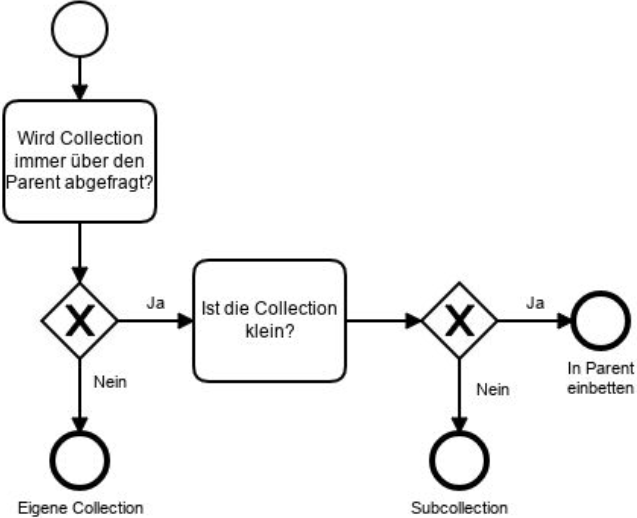
\includegraphics[width=0.6\linewidth]{img/nosql_one_to_many.png}

\subsubsection{NoSQL Many-To-Many}
\begin{itemize}
    \item Wie in relationaler Datenbank mit Assoziationstabelle
    \begin{itemize}
        \item Kein kopieren von Daten
        \item Komplexere Abfragen, keine Joins im Firestore
    \end{itemize}
    \item Oder Daten kopieren und einbetten
\end{itemize}
\textbf{Kopieren der Daten:} muss kein Nachteil sein.
Preisänderung eines Produktes hat keinen Einfluss auf vergangene Bestellungen.
Adressänderung eines Kunden verändert keine alten Bestellungen.
Kopierte Daten können mittels Trigger und Cloud Function wieder synchronisiert werden.